% 页面设置
\documentclass[12pt, a4paper]{article} % 字号:12,纸张:A4
\usepackage[top=2.54cm, bottom=2.54cm, left=3.18cm,right=3.18cm]{geometry} % 页边距设置
% 字体设置
\usepackage[UTF8]{ctex}
\usepackage{fontspec} % 设置字体
%\setCJKmainfont{SimSun}[AutoFakeBold=true, BoldFont={SimHei}, ItalicFont={KaiTi}] % 正文字体
%\setCJKsansfont[AutoFakeBold=3]{KaiTi} % 无衬线字体
%\setCJKmonofont[AutoFakeBold=3]{SimHei} % 等宽字体
\setmainfont{Times New Roman} % 设置主字体为新罗马体
% 文本设置
\usepackage{enumerate} % 支持小标题编号
\linespread{1.5} % 行间距1.5倍
\usepackage{indentfirst}%首段缩进
\setlength{\parindent}{2em} % 首行缩进两字符
\usepackage[hidelinks]{hyperref} % 目录添加超链接
\usepackage{zhnumber} % 章节标题中文显示
\usepackage[cmyk]{xcolor} % 文字彩色显示
% 数学支持
\usepackage{amsmath} % 数学公式支持
\usepackage{amssymb} % 数学符号支持
\usepackage{bm} % 公式加粗
\usepackage{mathrsfs} % 花体字母
\usepackage{yhmath} % 更多的数学符号
% 图片设置
\usepackage{caption} % 插入图片标题
\usepackage{float} % 控制图片位置
\usepackage{subfigure} % 图片并排
\usepackage{booktabs} % 插入表格
% 表格设置
\usepackage{multirow} % 表格自动换行
\usepackage{bigstrut} % 表格间距
\usepackage{rotating} % 表格旋转
\usepackage{tabularx} % 表格宽度
\usepackage{colortbl} % 表格颜色
\usepackage{graphicx} % 表格自动宽度

\title{第二章 \ \ \ 线性模型} % 文章标题
\author{Castor Ye} % 文章作者
\date{} % 文章时间

\begin{document} % 文档从这里开始。
\maketitle % 按照预定的模板把上面那些信息排好。
\newtheorem{definition}{定义}[section]
\newtheorem{theorem}{定理}[section]
\newtheorem{example}{例}[section]
\newtheorem{solution}{题解}
\newtheorem{algorithm}{算法}
\newtheorem{axiom}{公理}
\newtheorem{property}{性质}
\newtheorem{proposition}{命题}
\newtheorem{lemma}{引理}
\newtheorem{corollary}{推论}[section]
\newtheorem{remark}{注解}
\newtheorem{condition}{条件}
\newtheorem{conclusion}{结论}
\newtheorem{assumption}{假设}
\renewcommand{\figurename}{图} % 将图片序号改为图
\renewcommand{\tablename}{表} % 将表格序号改为表
%%%%%%%%%%%%%%%%%%%%%%%%%%%%%%%%%%%%%%%%%%%%%%%%%%%%%%%%%%%%%%%%%%%%%%%
% 文章内容从此开始
\section{基本形式}

给定由 $d$ 个属性描述的示例 $x = (x_1; x_2; \cdots; x_d)$,其中 $x_i$ 是 $x$ 在第 $i$ 个属性上的取值,线性模型(linear model)试图学得一个通过属性的线性组合来进行预测的函数,即:
\begin{equation*}
    f(x) = w_1x_1 + w_2x_2 + \cdots + w_dx_d + b
\end{equation*}

一般用向量形式写成:
\begin{equation*}
    f(x) = w^T x + b
\end{equation*}
其中 $w = (w_1; w_2; \cdots ; w_d)$,$w$ 和 $b$ 学得之后,模型就得以确定。

\section{线性回归}

给定数据集 $D = \{(x_1, y_2), (x_2, y_2), \cdots, (x_m, y_m)\}, x_i = (x_{i1}; x_{i2}; \cdots; x_{id}), y_i \in \mathbb{R}$。“线性回归”(linear regression)试图学得一个线性模型以尽可能准确地预测实值输出标记。例如:根据历年城市 GDP 预测未来 GDP,或者根据历年天气数据预测今年农作物收成等。

对于连续值的属性,一般都可以直接或经过预处理(归一化等)后被学习器所用。但对于离散值,我们可以做以下处理:

\begin{enumerate}[\hspace*{2em} i.]
    \item 若属性间存在“序”(order)关系,可通过连续化将其转化为连续值。例如:身高属性分为“高”“中”“矮”,可转化为数值:$\{1, 0.5, 0\}$。
    \item 若属性间不存在“序”(order)关系,则通常将其转化为向量的形式。例如:性别属性分为“男”“女”,可转化为二维向量:${(1, 0), (0, 1)}$。
\end{enumerate}

线性回归试图学得:
\begin{equation*}
    f(x_i) = wx_i + b, \ \ \text{使得} f(x_i) \simeq y_i
\end{equation*}

为了确定 $w$ 和 $b$,我们可以引入均方误差:
\begin{equation*}
    \begin{array}{*{20}{l}}
        {({w^*},{b^*})}&{ = \mathop {\arg \min }\limits_{(w,b)} \sum\limits_{i = 1}^m {{{(f({x_i}) - {y_i})}^2}} }\\
        {}&{ = \mathop {\arg \min }\limits_{(w,b)} \sum\limits_{i = 1}^m {{{({y_i} - w{x_i} - b)}^2}} }
    \end{array}
\end{equation*}

均方误差有非常好的几何意义,它对应了常用的“欧几里得距离(两点直线距离)”(Euclidean distance)。基于均方误差最小化来进行模型求解的方法称为“最小二乘法”(least square method)。在线性回归中,最小二乘法就是试图找到一条直线,使所有样本到直线上的欧氏距离之和最小。

求解 $w$ 和 $b$ 使 $\displaystyle E_{(w, b)} = \sum_{i = 1}^{m} (y_i - wx_i -b)^2$ 最小化的过程,称为线性回归模型的最小二乘“参数估计”(parameter estimation)。我们可将 $E_{(w, b)}$ 分别对 $w$ 和 $b$ 求导,得到:
\begin{equation*}
    \frac{{\partial {E_{(w,b)}}}}{{\partial w}} = 2\left( {w\sum\limits_{i = 1}^m {x_i^2}  - \sum\limits_{i = 1}^m {({y_i} - b){x_i}} } \right)
\end{equation*}
\begin{equation*}
    \frac{{\partial {E_{(w,b)}}}}{{\partial b}} = 2\left( {mb - \sum\limits_{i = 1}^m {({y_i} - w{x_i})} } \right)
\end{equation*}

令上面两式为零可得到 $w$ 和 $b$ 最优解的闭式(closed-form)解:
\begin{equation*}
    w = \frac{{\sum\limits_{i = 1}^m {{y_i}\left( {{x_i} - \bar x} \right)} }}{{\sum\limits_{i = 1}^m {x_i^2}  - \frac{1}{m}{{\left( {\sum\limits_{i = 1}^m {{x_i}} } \right)}^2}}} \ \ \ b = \frac{1}{m}\sum\limits_{i = 1}^m {({y_i} - w{x_i})}
\end{equation*}
其中 $\displaystyle \bar{x} = \frac{1}{m} \sum_{i = 1}^{m} x_i$,为 $x$ 的均值。

注意:
\begin{enumerate}[\hspace*{2em} i.]
    \item 这里 $E_{(w, b)}$ 是关于 $w$ 和 $b$ 的凸函数,当它关于 $w$ 和 $b$ 的导数均为零时,得到 $w$ 和 $b$ 的最优解。
    \item 对区间 $[a, b]$ 上定义的函数 $f$,若该函数对区间中任意两点 $x_1, x_2$ 均有 $\displaystyle f(\frac{x_1 + x_2}{2}) \le \frac{f(x_1) + f(x_2)}{2}$,则称 $f$ 为区间 $[a, b]$ 上的凸函数。
    \item 对实数集上的函数,可以通过求二阶导数来判别:若二阶导数在区间上非负,则称为凸函数;若二阶导在区间上恒大于零,则为严格凸函数。
\end{enumerate}

更一般的情形是如本节开头的数据集 $D$,样本由 $d$ 个属性描述,此时我们试图学得:
\begin{equation*}
    f(x_i) = w^T x_i + b_i, \ \ \ \text{使得} f(x_i) \simeq y_i
\end{equation*}
这称为“多元线性回归”(multivariate linear regression)。

类似的,可利用最小二乘法来对 $w$ 和 $b$ 进行估计。为便于讨论,我们把 $w$ 和 $b$ 吸收入向量形式 $\hat{w} = (w; b)$,相应的,把数据集 $D$ 表示为一个 $m \times (d + 1)$ 大小的矩阵 $X$,其中每行对应于一个示例,该行前 $d$ 个元素对应于示例的 $d$ 个属性值,最后一个元素恒置为 $1$,即:
\begin{equation*}
    \hat w = (w;b) = {\left[ {\begin{array}{*{20}{c}}
        {{w_1}}&{{w_2}}& \cdots &{{w_d}}&b
    \end{array}} \right]^T}
\end{equation*}
\begin{equation*}
    X = \left[ {\begin{array}{*{20}{c}}
        {{x_{11}}}&{{x_{12}}}& \cdots &{{x_{1d}}}&1\\
        {{x_{21}}}&{{x_{22}}}& \cdots &{{x_{2d}}}&1\\
         \vdots & \vdots & \ddots & \vdots & \vdots \\
        {{x_{m1}}}&{{x_{m2}}}& \cdots &{{x_{md}}}&1
        \end{array}} \right] = \left[ {\begin{array}{*{20}{c}}
        {x_1^T}&1\\
        {x_2^T}&1\\
         \vdots & \vdots \\
        {x_m^T}&1
    \end{array}} \right]
\end{equation*}
\begin{equation*}
    X \cdot \hat w = \left[ {\begin{array}{*{20}{c}}
        {{w_1}{x_{11}} + {w_2}{x_{12}} +  \cdots  + {w_d}{x_{1d}} + b}\\
        {{w_1}{x_{21}} + {w_2}{x_{22}} +  \cdots  + {w_d}{x_{2d}} + b}\\
         \cdots \\
        {{w_1}{x_{m1}} + {w_2}{x_{m2}} +  \cdots  + {w_d}{x_{md}} + b}
        \end{array}} \right] = \left[ {\begin{array}{*{20}{c}}
        {f\left( {{x_1}} \right)}\\
        {f\left( {{x_2}} \right)}\\
         \cdots \\
        {f\left( {{x_m}} \right)}
    \end{array}} \right]
\end{equation*}
再把标记也写成向量形式 $y = (y_1; y_2; \cdots; y_m)$,则有:
\begin{equation*}
    \hat{w}^* = \mathop {\arg \min }\limits_{\hat w} {\left( {y - X\hat w} \right)^T}\left( {y - X\hat w} \right)
\end{equation*}

令 $E_{\hat{w}} = {\left( {y - X\hat w} \right)^T}\left( {y - X\hat w} \right)$,对 $\hat{w}$ 求导得到:
\begin{equation*}
    \frac{{\partial {E_{\hat w}}}}{{\partial \hat w}} = 2{X^T}(X\hat w - y)
\end{equation*}
令上式为零可得 $\hat{w}$ 最优解的闭式解,但由于涉及矩阵逆的计算,比单变量情形要复杂一些,下面做一个简单讨论:

当 $X^TX$ 为满秩矩阵(full-rank matrix)或正定矩阵(positive definite matrix)时,即矩阵行列式不为零时,令上式为零得到:
\begin{equation*}
    \hat{w}^* = (X^TX)^{-1} X^T y
\end{equation*}
其中 $(X^TX)^{-1}$ 是矩阵 $(X^TX)$ 的逆矩阵。令 $\hat{x}_i = (x_i, 1)$,则最终学得的多元线性回归模型为:
\begin{equation*}
    f(\hat{x}_i) = \hat{x}_i^T (X^TX)^{-1} X^Ty
\end{equation*}

对于非满秩矩阵,我们不进行深入。

另一方面,有时候原始的线性回归并不能满足需求。例如:$y$ 并不是线性变化,而是指数变化。此时我们可以采用线性模型来逼近 $y$ 的衍生物,例如 $\ln y$,如下图所示。这就是“对数线性回归”(log-linear regression),它实际上是在试图让 $e^{w^Tx +b}$ 逼近 $y$。

\begin{figure}[H]
    \centering
    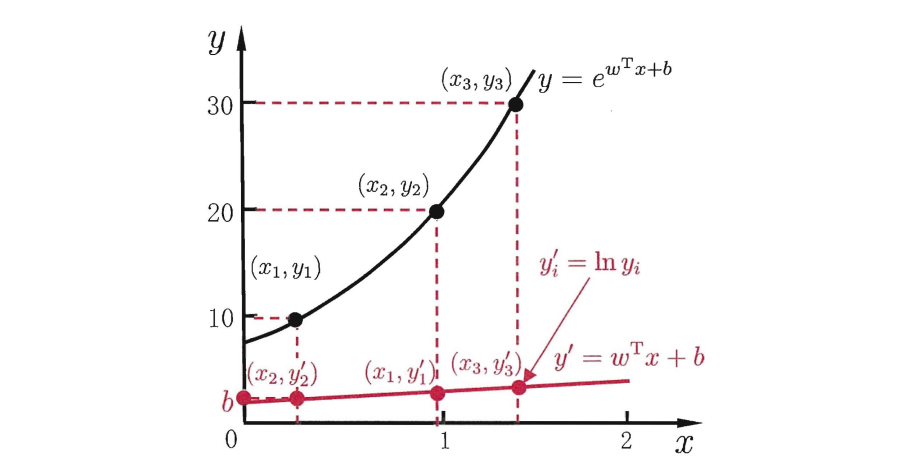
\includegraphics[width=0.8\textwidth]{../img/3-1-对数线性回归示意图.png}
    \caption{对数线性回归示意图}
    \label{fig:对数线性回归示意图}
\end{figure}

更一般得,考虑单调可微函数 $g(\cdot)$,令:
\begin{equation*}
    y = g^{-1} (w^T x + b)
\end{equation*}
这样得到的模型称为“广义线性模型”(generalized linear model),其中函数 $g(\cdot)$ 称为“联系函数”(link function)。

\section{对数几率回归}

回归就是通过输入的属性值得到一个预测值,利用上述广义线性模型的特征,是否可以通过一个联系函数,将预测值转化为离散值从而进行分类呢?线性几率回归正是研究这样的问题。

对于二分类问题,我们希望找到一个可以将连续值转化为离散值,并且单调可微的函数。对数几率引入了一个对数几率函数(logistic function),将预测值投影到 $0-1$ 之间,从而将线性回归问题转化为二分类问题。
\begin{equation*}
    y = \frac{1}{1 + e^{-z}}
\end{equation*}

\begin{figure}[H]
    \centering
    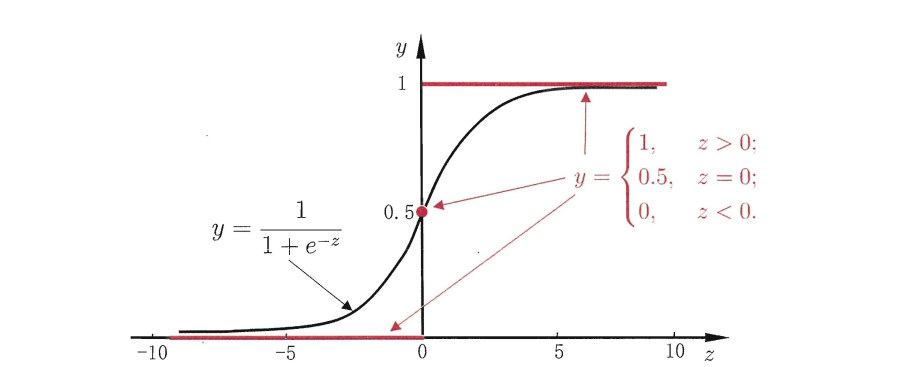
\includegraphics[width=0.8\textwidth]{../img/3-2-单位阶跃函数与对数几率函数.png}
    \caption{单位阶跃函数与对数几率函数}
    \label{fig:单位阶跃函数与对数几率函数}
\end{figure}

从上图可以看出,对数几率函数是一种“$Sigmoid$ 函数”,它将 $z$ 值转化为一个接近 $0$ 或 $1$ 的 $y$ 值,并且其输出在 $z = 0$ 附近变化很陡。将对数几率函数作为 $g^-(\cdot)$ 代入 $y = g^{-1} (w^T x + b)$ 可以得到:
\begin{equation*}
    y = \frac{1}{1 + e^{- (w^T x + b)}} \Rightarrow \ln \frac{y}{1 - y} = w^Tx + b
\end{equation*}

若将 $y$ 视为样本 $x$ 作为正例的可能性,则 $1 - y$ 是其反例可能性,两者的比值:
\begin{equation*}
    \frac{y}{1 - y}
\end{equation*}
称为“几率”(odds),反映了 $x$ 作为正例的相对可能性,对几率取对数则得到“对数几率”(log odds,亦称 logit):
\begin{equation*}
    \ln \frac{y}{1 - y}
\end{equation*}

由此看出,该模型实际上是在用线性回归模型的预测结果去逼近真实标记的对数几率,因此,其对应的模型称为“对数几率回归”(logistic regression,亦称 logit regression)。

下面使用“极大似然法”(maximum likelihood method)来估计 $w$ 和 $b$,首先我们将 $y$ 视为类后验概率估计 $p(y = 1 | x)$,则有:
\begin{equation*}
    \ln \frac{{p(y = 1|x)}}{{p(y = 0|x)}} = {w^T}x + b \Rightarrow \left\{ \begin{array}{l}
        \displaystyle p(y = 1|x) = \frac{{{e^{{w^T}x + b}}}}{{1 + {e^{{w^T}x + b}}}}\\
        \displaystyle p(y = 0|x) = \frac{1}{{1 + {e^{{w^T}x + b}}}}
    \end{array} \right.
\end{equation*}

然后,给定数据集 $\{(x_i, y_i)\}_{i = 1}^{m}$,对率回归模型最大化“对数似然”(log-likelihood):
\begin{equation*}
    \ell (w,b) = \sum\limits_{i = 1}^m {\ln p({y_i}|{x_i};w,b)}
\end{equation*}

\section{线性判别分析}

线性判别分析(Linear Discriminant Analysis, LDA)是一种经典的线性学习方法,也称“Fisher判别分析”。LDA 的基本思想是:给定训练样例集,设法将样例投影到一条直线上,使得同类样例的投影点尽可能接近、异类样例的投影点尽可能远离;在对新样本进行分类时,将其投影到同样的这条直线上,再根据投影点的位置来确定新样本的类别。

\begin{figure}[H]
    \centering
    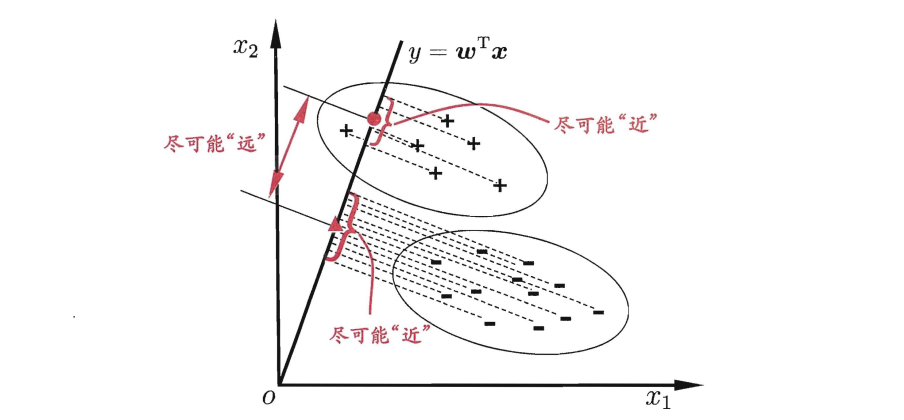
\includegraphics[width=0.8\textwidth]{../img/3-3-LDA的二维示意图.png}
    \caption{LDA 的二维示意图,“$+, -$”分别代表正例和反例,椭圆表示数据簇的外轮廓,虚线表示投影,红色实心圆和实心三角形分别表示两类样本投影后的中心点}
    \label{fig:label}
\end{figure}

给定数据集 $D = \{(x_i, y_i)\}_{i = 1}^{m}, y_i \in \{0, 1\}$,令 $X_i, \mu_i, \sum_i$ 分别表示第 $i \in \{0, 1\}$ 类示例的集合、均值向量、协方差矩阵。若将数据投影到直线 $w$ 上,则两类样本的中心在直线上的投影分别为 $w^T\mu_0$ 和 $w^T \mu_1$;若将所有样本点都投影到直线上,则两类样本的协方差分别为 $w^T \sum_0 w$ 和 $w^T \sum_1 w$。由于直线是一维空间,因此 $w^T\mu_0, w^T \mu_1, w^T \sum_0 w, w^T \sum_1 w$ 均为实数。

为了让同类样本的投影点尽可能接近,不同类样本点投影之间尽可能远离,即:让同类的协方差之和尽可能小,类中心之间的距离尽可能大。

定义“类内散度矩阵”(within-class scatter matrix),越小越好:
\begin{equation*}
    \begin{array}{*{20}{l}}
        {{S_w}}&{ = {\sum _0} + {\sum _1}}\\
        {}&{ = \sum\limits_{x \in {X_0}} {(x - {\mu _0}){{(x - {\mu _0})}^T}}  + \sum\limits_{x \in {X_1}} {(x - {\mu _1}){{(x - {\mu _1})}^T}} }
    \end{array}
\end{equation*}

“类间散度矩阵”(between-class scatter matrix),越大越好:
\begin{equation*}
    S_b = (\mu_0 - \mu_1)(\mu_0 - \mu_1)^T
\end{equation*}

因此得到 LDA 的最大化目标:“广义瑞利商”(generalized Rayleigh quotient):
\begin{equation*}
    J = \frac{w^T S_b w}{w^T S_w w}
\end{equation*}

从而分类问题转化为最优化求解 $w$ 的问题,当求解出 $w$ 后,对新的样本进行分类时,只需将样本点投影到这条直线上,根据与各个类别的中心值进行比较,从而判定储新样本与哪个类别距离最近。求解 $w$ 的方法如下所示,使用方法为拉格朗日乘子法:
\begin{equation*}
    \left. \begin{array}{l}
        \mathop {\min }\limits_w \ \ \  - {w^T}{S_b}w\\
        s.t. \ \ \ {w^T}{S_w}w = 1
    \end{array} \right\}{S_b}w = \lambda {S_w}w
\end{equation*}
解只与 $w$ 的方向有关,与长度无关。注意到 $S_b w$ 的方向恒为 $\mu_0 - \mu_1$,则令 $S_b w = \lambda (\mu_0 - \mu_1)$,代入得:
\begin{equation*}
    w = S_w^{-1} (\mu_0 - \mu_1)
\end{equation*}

若将 $w$ 看做一个投影矩阵,类似 PCA 的思想,则 LDA 可将样本投影到 $N-1$ 维空间($N$ 为类簇数),投影的过程使用了类别信息(标记信息),因此 LDA 也常被视为一种经典的监督降维技术。

\section{多分类学习}

现实中我们经常遇到不只两个类别的分类问题,即多分类问题,在这种情形下,我们常常运用“拆分”的策略,通过多个二分类学习器来解决多分类问题,即将多分类问题拆解为多个二分类问题,训练出多个二分类学习器,最后将多个分类结果进行集成得出结论。最为经典的拆分策略有三种:“一对一”($OvO$)、“一对其余”($OvR$)和“多对多”($MvM$),核心思想与示意图如下所示。

\begin{enumerate}[\hspace*{2em} i.]
    \item $OvO$:给定数据集 $D$ ,假定其中有N个真实类别,将这N个类别进行两两配对(一个正类/一个反类),从而产生 $N(N-1)/2$ 个二分类学习器,在测试阶段,将新样本放入所有的二分类学习器中测试,得出 $N(N-1)$个结果,最终通过投票产生最终的分类结果。
    \item $OvR$:给定数据集 $D$,假定其中有N个真实类别,每次取出一个类作为正类,剩余的所有类别作为一个新的反类,从而产生 $N$ 个二分类学习器,在测试阶段,得出 $N$ 个结果,若仅有一个学习器预测为正类,则对应的类标作为最终分类结果。
    \item $MvM$:给定数据集 $D$,假定其中有 $N$ 个真实类别,每次取若干个类作为正类,若干个类作为反类(通过ECOC码给出,编码),若进行了 $M$ 次划分,则生成了 $M$ 个二分类学习器,在测试阶段(解码),得出 $M$ 个结果组成一个新的码,最终通过计算海明(欧式)距离选择距离最小的类别作为最终分类结果。
\end{enumerate}

\begin{figure}[H]
    \centering
    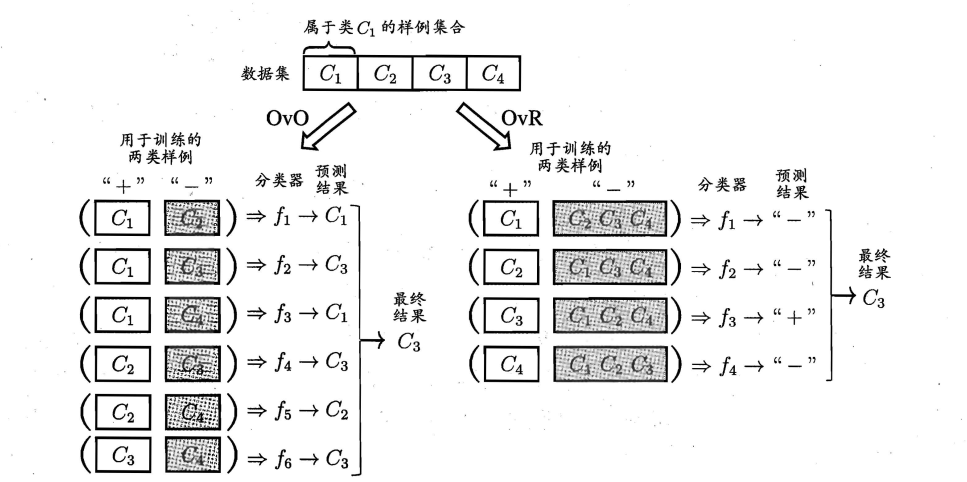
\includegraphics[width=0.8\textwidth]{../img/3-4-OvO与OvR示意图.png}
    \caption{OvO与OvR示意图}
    \label{fig:OvO与OvR示意图}
\end{figure}

\begin{figure}[H]
    \centering
    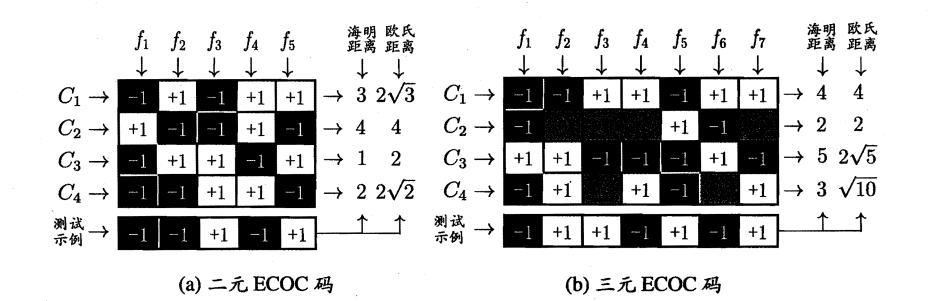
\includegraphics[width=0.8\textwidth]{../img/3-5-ECOC编码示意图.png}
    \caption{ECOC编码示意图}
    \label{fig:ECOC编码示意图,“$+1, -1$”分别表示学习器 $f_i$ 将该类样本作为正、反例;三元码中“$0$”表示 $f_i$ 不使用该类样本}
\end{figure}


\end{document}